%\iffalse
\let\negmedspace\undefined
\let\negthickspace\undefined
\documentclass[journal,12pt,twocolumn]{IEEEtran}
\usepackage{cite}
\usepackage{amsmath,amssymb,amsfonts,amsthm}
\usepackage{algorithmic}
\usepackage{graphicx}
\usepackage{textcomp}
\usepackage{xcolor}
\usepackage{txfonts}
\usepackage{listings}
\usepackage{enumitem}
\usepackage{mathtools}
\usepackage{gensymb}
\usepackage{comment}
\usepackage[breaklinks=true]{hyperref}
\usepackage{tkz-euclide} 
\usepackage{listings}
\usepackage{gvv}                                        
\def\inputGnumericTable{}                                 
\usepackage[latin1]{inputenc}                                
\usepackage{color}                                            
\newtheorem{theorem}{Theorem}[section]
\usepackage{array}                                            
\usepackage{longtable}                                       
\usepackage{calc}                                             
\usepackage{multirow}                                         
\usepackage{hhline}                                           
\usepackage{ifthen}                                           
\usepackage{lscape}
\newtheorem{problem}{Problem}
\newtheorem{proposition}{Proposition}[section]
\newtheorem{lemma}{Lemma}[section]
\newtheorem{corollary}[theorem]{Corollary}
\newtheorem{example}{Example}[section]
\newtheorem{definition}[problem]{Definition}
\newcommand{\BEQA}{\begin{eqnarray}}
\newcommand{\EEQA}{\end{eqnarray}}
\newcommand{\define}{\stackrel{\triangle}{=}}
\theoremstyle{remark}
\newtheorem{rem}{Remark}
\begin{document}
\bibliographystyle{IEEEtran}
\vspace{3cm}
\title{GATE: IN/28}
\author{EE23BTECH11040 - Manoj Kumar Ambatipudi$^{*}$% <-this % stops a space
}
\maketitle
\newpage
\bigskip
\renewcommand{\thefigure}{\theenumi}
\renewcommand{\thetable}{\theenumi}
\textbf{QUESTION:}
Consider the discrete time signal $x\sbrak{n} = u\sbrak{-n+5} - u\sbrak{n+3}$, where
\[u\sbrak{n} = 
\begin{cases}
    1;n\geq0\\
    0;n<0
\end{cases}
\]
The smallest n for which $x\sbrak{n} = 0$ is?\\
\textbf{Solution:}
$x\brak{n}$ can be defined as 
\begin{align}
    x\brak{n} = h\brak{n} - f\brak{n}
\end{align}
Where 
\begin{align}
    h\brak{n} &= u\brak{-n+5}\\
    f\brak{n} &= u\brak{n+3}
\end{align}
Find the values of n for which 
\begin{align}
    h(n) = f(n)
\end{align}
Using \figref{IN/28/fig_2} to get the values of n, the range of n is given as
\begin{align*}
    n \in [-3,5]
\end{align*}
Hence the lowest value of n 
\begin{align}
    \boxed{n = -3}
\end{align}
\begin{figure}[h!]
\renewcommand\thefigure{1}
    \centering
    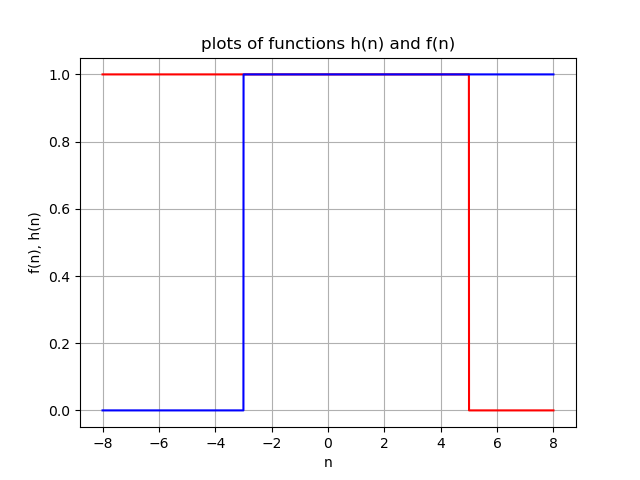
\includegraphics[width = 1.0\columnwidth]{fig_2.png}
    \caption{Plots of h(n), f(n) taken from python3}
    \label{IN/28/fig_2}
\end{figure}
\begin{figure}[h!]
\renewcommand\thefigure{2}
    \centering
    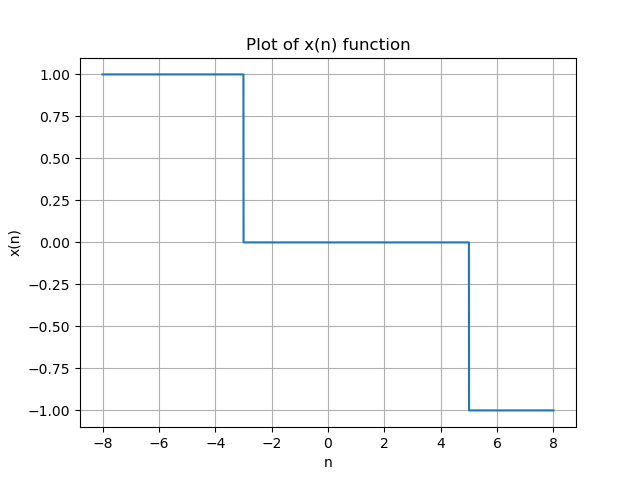
\includegraphics[width = 1.0\columnwidth]{fig_1.png}
    \caption{Plot of function x\brak{n} taken from Python3}
    \label{fig:enter-label}
\end{figure}
\end{document}
